\documentclass[A4,svgnames,9pt,aspectratio=169]{beamer}
%% document options:
%% - aspectratio = { 43, 169, 1610 }
%% - utf8
%%

%%
%% insert list of packages
%%

%% \usepackage[english,french]{babel}

\hypersetup{ 
   allcolors=blue_eut,
   pdfauthor   = {Nathan Davouse},
   pdftitle    = {\@title},
   pdfsubject  = {Optimisation, LLM},
   pdfkeywords = {Internship, Defence}
}

%%%%%%%%%%%%%%%%%%%%%%%%%%%%%%%%%%%%%%%%%%%%%%%%%%%%%%%
%%
%%%%%%%%%%%%%%%%%%%%%%%%%%%%%%%%%%%%%%%%%%%%%%%%%%%%%%%
\usepackage{blindtext}
\usepackage{appendixnumberbeamer}
\usepackage[absolute,overlay]{textpos}
\usepackage{multirow}
\usepackage{tikz}
\usetikzlibrary{calc,shapes, arrows, positioning, fit, backgrounds}

\title[titrecourt]{Optimization des Hyperparamètres appliquée au Fine Tuning de LLM}
\subtitle{Basé sur l'article : \textit{Bayesian and Partition-Based Optimization for Hyperparameter Optimization of LLM Fine-Tuning}}
\date[19/02/2025]{date long}
\author[A. et al.]{Nathan Davouse}
\newcommand{\semester}{A24}
\newcommand{\course}{Soutenance ST30}


\usetheme{utt}

\begin{document}

% Appeler la page titre
\frame{\titlepage}

% Renommer le titre du sommaire, pour une présentation en anglais par exemple
\renewcommand{\contentsname}{Sommaire}
% Appeler la page de sommaire
%\frame{\tocpage}

%%%%%%%%%%%%%%%%%%%%%%%%%%%%%%%%%%%%%%%%%%%%%%%%%%%%%%%
\section{Introduction}
\begin{frame}{Large Language Model (LLM)}
   
\end{frame}

\begin{frame}{Fine Tuning}
   
\end{frame}

\begin{frame}{Hyperparameter Optimization}
   
\end{frame}

\begin{frame}{Problem Formulation}
   
\end{frame}

\begin{frame}{Related Works}
   
\end{frame}
%%%%%%%%%%%%%%%%%%%%%%%%%%%%%%%%%%%%%%%%%%%%%%%%%%%%%%%

%%%%%%%%%%%%%%%%%%%%%%%%%%%%%%%%%%%%%%%%%%%%%%%%%%%%%%%
\section{Design et Implémentation}
\begin{frame}{Search Space}
    
\end{frame}

\begin{frame}{Search Strategy : BO}

\end{frame}

\begin{frame}{Search Strategy : SOO}

\end{frame}

\begin{frame}{Search Strategy : BaMSOO}

\end{frame}

\begin{frame}{Performance Estimation Strategy}

\end{frame}

\begin{frame}{Implémentation}

\end{frame}

%%%%%%%%%%%%%%%%%%%%%%%%%%%%%%%%%%%%%%%%%%%%%%%%%%%%%%%

%%%%%%%%%%%%%%%%%%%%%%%%%%%%%%%%%%%%%%%%%%%%%%%%%%%%%%%
\section{Résultats et Analysis}
%%%%%%%%%%%%%%%%%%%%%%%%%%%%%%%%% LHS results %%%%%%%%%%%%%%%%%%
\begin{frame}{Echantillonnage par Latin Hypercube Sampling (LHS)}
    \begin{block}{}
        Objectif : Explorer l'espace et proposer une borne inférieure
        
    \end{block}\vspace*{-10pt}
    \begin{columns}
        %%%%%%%%%%%%%%%%%%%%%%%%%% COLONNE DE GAUCHE %%%%%%%%%%%%%%
        \begin{column}{0.35\textwidth} 

            \begin{figure}
                \centering
                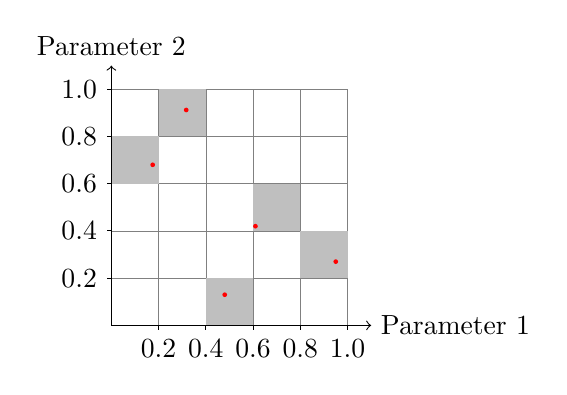
\begin{tikzpicture}[scale=3]

    % Define the grid
    \draw[step=0.2,gray,very thin] (0,0) grid (1,1);
    
    % Shade specific squares
    \fill[gray!50] (0.0,0.6) rectangle (0.2,0.8);
    \fill[gray!50] (0.2,0.8) rectangle (0.4,1.0);
    \fill[gray!50] (0.4,0.0) rectangle (0.6,0.2);
    \fill[gray!50] (0.6,0.4) rectangle (0.8,0.6);
    \fill[gray!50] (0.8,0.2) rectangle (1.0,0.4);
    
    % Draw red points
    \fill[red] (0.175,0.68) circle (0.01);  % Point in the first square
    \fill[red] (0.317,0.912) circle (0.01);  % Point in the second square
    \fill[red] (0.48,0.13) circle (0.01);  % Point in the third square
    \fill[red] (0.61,0.42) circle (0.01);  % Point in the fourth square
    \fill[red] (0.95,0.27) circle (0.01);  % Point in the fifth square
    
    % Draw the axes
    \draw[->] (0,0) -- (1.1,0) node[right] {Parameter 1};
    \draw[->] (0,0) -- (0,1.1) node[above] {Parameter 2};
    
    % Add ticks and labels
    \foreach \x in {0.2,0.4,0.6,0.8,1.0} {
      \draw (\x,0) -- (\x,-0.02) node[below] {\x};
      \draw (0,\x) -- (-0.02,\x) node[left] {\x};
    }
    
\end{tikzpicture}
                \caption{Illustration du Latin Hypercube Sampling avec $g=5$}
            \end{figure} 
     
            \end{column}
                 
         %%%%%%%%%%%%%%%%%%%%%%%%% COLONNE DE DROITE %%%%%%%%%%%%%%
            \begin{column}{0.55\textwidth}
                \begin{figure}
                    \centering
                    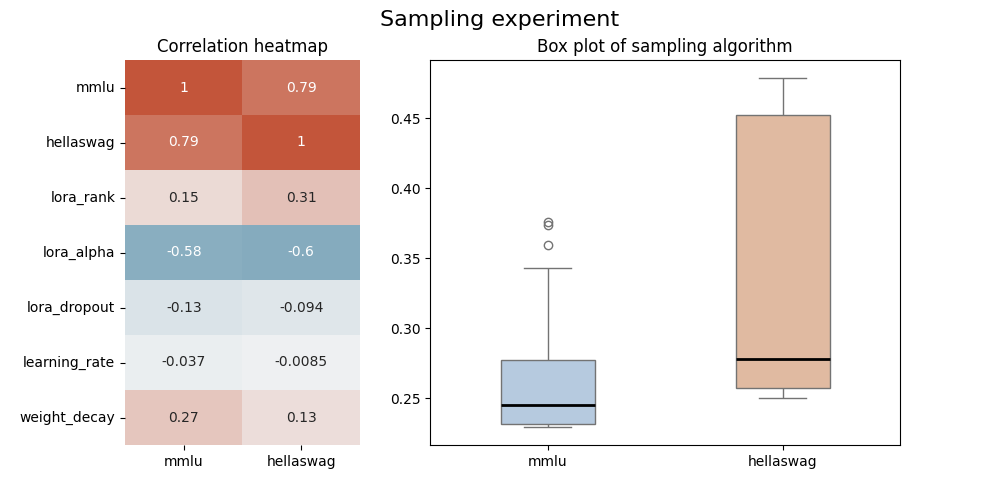
\includegraphics[width = \textwidth]{assets/imgs/plots/sampling/lhs.png}
                    \vspace*{-20pt}\caption{Résumé des résultats par sampling}
                \end{figure} 
            \end{column}
                 
    \end{columns}
\end{frame}

%%%%%%%%%%%%%%%%%%%%%%%%%%%%%%%%% Résultats %%%%%%%%%%%%%%%%%%
\begin{frame}{Résultats des 3 algorithms}
    \begin{columns}
        \begin{column}{0.45\textwidth}
            \begin{figure}
                \centering
                \begin{tikzpicture}[domain = 0:50,scale = 0.7]
    \tikzstyle{point} = [only marks, mark = triangle*, mark size = 3, opacity = 0.5]
    \begin{axis}[
        legend pos=south east,
        ymin = 0.2,
        x=3.2,
        y =700
    ]
    \addplot [blue,point, visible on = <1> ] table {assets/tikz_picture/global_results/bo_mmlu.dat};
    \addlegendentry{BO}

    \addplot [red, point, visible on = <2>] table {assets/tikz_picture/global_results/soo_mmlu.dat};
    \addlegendentry{SOO}

    \addplot [violet, point, visible on = <3>] table {assets/tikz_picture/global_results/bamsoo_mmlu.dat};
    \addlegendentry{BaMSOO}



    \addplot [blue,point, visible on = <4>] table {assets/tikz_picture/global_results/bo_mmlu.dat};
    \addplot [red, point, visible on = <4>] table {assets/tikz_picture/global_results/soo_mmlu.dat};
    \addplot [violet, point, visible on = <4>] table {assets/tikz_picture/global_results/bamsoo_mmlu.dat};




    \end{axis}
\end{tikzpicture}
                \caption{Résultats sur MMLU (test)}
            \end{figure}
        \end{column}
        \begin{column}{0.45\textwidth}
            \begin{figure}
                \centering
                \begin{tikzpicture}[domain = 0:50,scale = 0.7]
    \tikzstyle{point} = [only marks, mark = triangle*, mark size = 3, opacity = 0.5]
    \begin{axis}[
        legend pos=south east,
        ymin = 0.2,
        x=3.2,
        y =450
    ]
    \addplot [blue,point, visible on = <1>] table {assets/tikz_picture/global_results/bo_hellaswag.dat};
    \addlegendentry{BO}

    \addplot [violet, point, visible on = <2>] table {assets/tikz_picture/global_results/bamsoo_hellaswag.dat};
    \addlegendentry{BaMSOO}

    \addplot [red, point, visible on = <3>] table {assets/tikz_picture/global_results/soo_hellaswag.dat};
    \addlegendentry{SOO}

    \addplot [blue,point, visible on = <4>] table {assets/tikz_picture/global_results/bo_hellaswag.dat};
    \addplot [violet, point, visible on = <4>] table {assets/tikz_picture/global_results/bamsoo_hellaswag.dat};
    \addplot [red, point, visible on = <4>] table {assets/tikz_picture/global_results/soo_hellaswag.dat};



    \end{axis}
\end{tikzpicture}
                \caption{Résultats sur Hellaswag (Validation)}
            \end{figure}
        \end{column}
    \end{columns}
\end{frame}

%%%%%%%%%%%%%%%%%%%%%%%%%%%%%%%%% Analyse %%%%%%%%%%%%%%%%%%
\begin{frame}{Analyse}
    \begin{table}[h!]
        \centering
        \begin{tabular}{|c||c|c||c|c|c|}
        \hline
           Jeu de données  & Borne Inf.$^1$& Borne Sup.$^2$ & BO-GP & SOO & BaMSOO \\
        \hline
           Hellaswag (validation)  & 47.90 & \textit{41.5} & \textbf{47.91} & 47.84 & 47.84\\
           MMLU (testing) & 37.61 & 49.3 & \textbf{38.11} & 37.42 & 37.50 \\
        \hline
        \end{tabular}
        \caption{Bornes et meilleurs résultats sur les 2 jeu de données}
    \end{table}
    \vspace*{-5pt}{\footnotesize 1 : expérience avec LHS; 2 : Fine tuning par Meta}

    \begin{block}{Points clés}     
    \end{block}
    
    \vspace*{-15pt}
    \begin{columns}
        
        %%%%%%%%%%%%%%%%%%%%%%%%%% COLONNE DE GAUCHE %%%%%%%%%%%%%%
        \begin{column}{0.45\textwidth} 
                \begin{itemize}
                    \item Borne Sup. sur Hellaswag non pertinente
                    \item Seul BO arrive au dessus de LHS
                    \item BaMSOO n'améliore que peu SOO
                \end{itemize}
        \end{column}  
         %%%%%%%%%%%%%%%%%%%%%%%%% COLONNE DE DROITE %%%%%%%%%%%%%%
            \begin{column}{0.45\textwidth}
                \begin{itemize}
                    \item principe de BaMSOO fonctionnel (visible annexe \ref{ap:bamsoo_results})
                    \item Espace de solution n'évolue que peu, le retravailler pour mesurer pleinement la performance des algorithmes
                \end{itemize}
            \end{column}          
    \end{columns}
    
\end{frame}

%%%%%%%%%%%%%%%%%%%%%%%%%%%%%%%%% Perspectives %%%%%%%%%%%%%%%%%%

\begin{frame}{Perspectives}
    \begin{columns}
        
        %%%%%%%%%%%%%%%%%%%%%%%%%% COLONNE DE GAUCHE %%%%%%%%%%%%%%
        \begin{column}[t]{0.45\textwidth} 
            \begin{block}{Poursuite du travail}
                \begin{itemize}
                    \item Retour sur l'article et présentation en conférence (si validation)
                    \item Elargissement de l'espace de recherche
                    \item Diversification sur les modèles/données
                \end{itemize}                
            \end{block}

        \end{column}  
         %%%%%%%%%%%%%%%%%%%%%%%%% COLONNE DE DROITE %%%%%%%%%%%%%%
            \begin{column}[t]{0.45\textwidth}
                \begin{block}{Généralisation hors LLM}
                    \textbf{Optimisation fractale parallèle enrichie par approche bayésienne\footnote[3]{\textit Parallel Bayesian-enhanced Fractals Optimization}}

                    \begin{itemize}
                        \item Généralisation 
                    \end{itemize}
                \end{block}
            \end{column}
        
                 
    \end{columns}
    
\end{frame}
%%%%%%%%%%%%%%%%%%%%%%%%%%%%%%%%%%%%%%%%%%%%%%%%%%%%%%%


%%%%%%%%%%%%%%%%%%%%%%%%%%%%%%%%%%%%%%%%%%%%%%%%%%%%%%% 
\section{Conclusion}
\begin{frame}{Conclusion}
    Une conclusion
\end{frame}


%%%%%%%%%%%%%%%%%%%%%%%%%%%%%%%%%%%%%%%%%%%%%%%%%%%%%%%

%% Le texte est modifiable en changeant \thankyou
%% \renewcommand{\thankyou}{Thank You.}
\frame{\merci}

\appendix
\begin{frame}{Annexes \ref{ap:llm_architecture} : Transformer architecture}
    \label{ap:llm_architecture}
    \begin{figure}
        \centering
        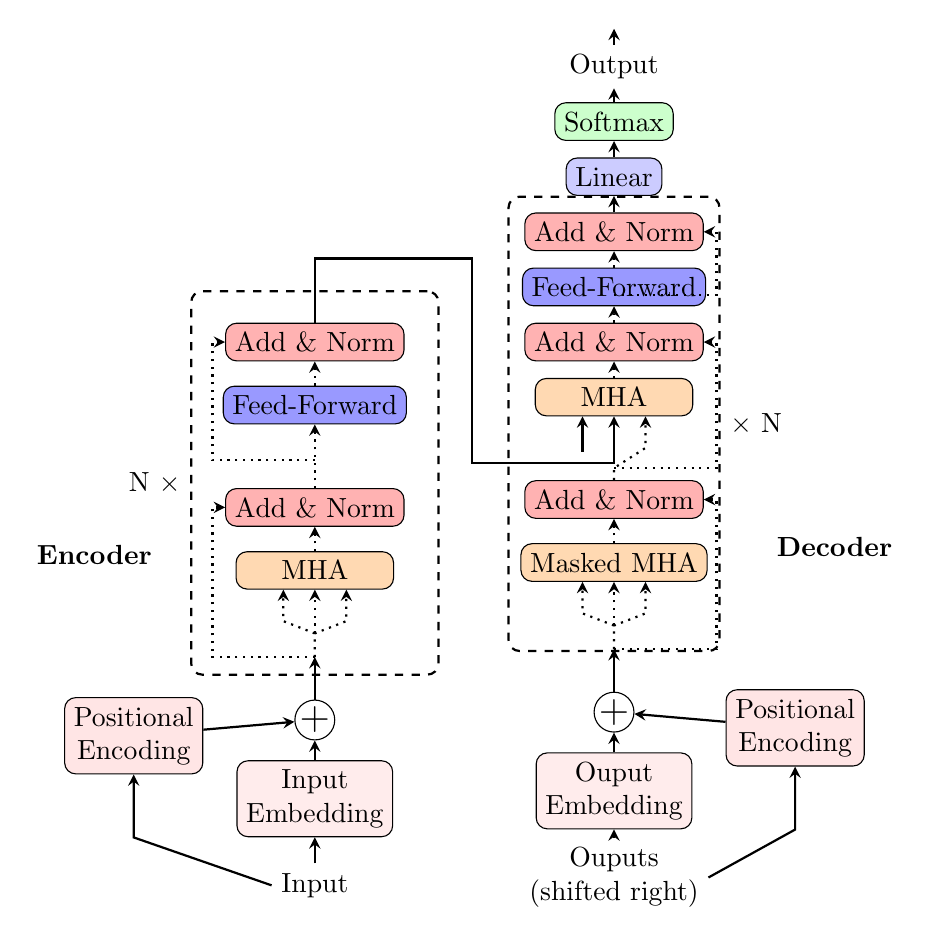
\begin{tikzpicture}[node distance=0.8cm]


    \tikzstyle{norm} = [rectangle, rounded corners, minimum width=1cm ,text centered, draw=black, fill=red!30]
    \tikzstyle{mha} = [rectangle,rounded corners, minimum width=2cm , text centered, draw=black, fill=orange!30]
    \tikzstyle{feed} = [rectangle, rounded corners, minimum width=1cm ,text centered, draw=black, fill=blue!40]
    \tikzstyle{embed} = [rectangle, rounded corners, minimum width=1cm ,text centered, draw=black, fill=pink!30]
    \tikzstyle{encoding} = [rectangle, rounded corners, minimum width=1cm ,text centered, draw=black, fill=pink!40]
    \tikzstyle{linear} = [rectangle, rounded corners, minimum width=1cm ,text centered, draw=black, fill=blue!20]
    \tikzstyle{softmax} = [rectangle, rounded corners, minimum width=1cm ,text centered, draw=black, fill=green!20]
    
    
    \tikzstyle{arrow} = [thick,->,>=stealth]
    \tikzstyle{lightA} = [thick,dotted,->,>=stealth]
    
    \tikzstyle{sum} = [circle, draw, minimum size=0.5cm, node distance=1cm, inner sep=0pt]
    
    % Decoder node
    
    \node (norm3)[norm,yshift = -0.5cm]{Add \& Norm};
    \node (feed2)[feed,below of = norm3, yshift = 0.1cm]{Feed-Forward};
    
    \node (norm4)[norm,below of = feed2,yshift=0.1cm]{Add \& Norm};
    \node (mha2)[mha,below of = norm4, yshift = 0.1cm]{MHA};
    
    \node (norm5)[norm,below of = mha2,yshift=-0.5cm]{Add \& Norm};
    \node (mha3)[mha,below of = norm5]{Masked MHA};
    
    % Encoder node
    
    \node (norm1)[norm,left of = norm4, xshift=-3cm]{Add \& Norm};
    \node (feed1)[feed,below of = norm1]{Feed-Forward};
    
    \node (norm2)[norm,below of = feed1,yshift=-0.5cm]{Add \& Norm};
    \node (mha1)[mha,below of = norm2]{MHA};
    
    % Arrow inside encoder
    \node (enc_base)[below of = mha1]{};
    
    \draw[lightA] (enc_base.center) -- (mha1);
    \draw[lightA] (enc_base.center) -- ([xshift=-0.4cm, yshift = -0.4cm]mha1.south) -- ([xshift=-0.4cm]mha1.south);
    \draw[lightA] ([yshift = -0.3cm]enc_base.center) -- (enc_base.center) -- ([xshift=0.4cm, yshift = -0.4cm]mha1.south) -- ([xshift=0.4cm]mha1.south);
    
    \draw[lightA] ([yshift = -0.3cm]enc_base.center) -- ([yshift = -0.3cm,xshift = -1.3cm]enc_base.center) -- ([xshift = -1.3cm]norm2.center) -- (norm2.west);
    
    \draw [lightA] (mha1) -- (norm2); 
    \draw [lightA] (norm2) -- (feed1); 
    \draw [lightA] (feed1) -- (norm1); 
    
    \draw[lightA] ([yshift = 0.6cm]norm2.center) -- ([xshift = -1.3cm,yshift = 0.6cm]norm2.center) -- ([xshift = -1.3cm]norm1.center) -- (norm1.west);
    
    \node(enc_fit)[draw, thick, dashed, rounded corners, fit=(norm1)(feed1)(norm2)(enc_base), inner sep=0.4cm, label=left:{N $\times$ }] {};
    
    % Arrow inside decoder
    \node (dec_base)[below of = mha3]{};
    
    \draw[lightA] (dec_base.center) -- (mha3);
    \draw[lightA] (dec_base.center) -- ([xshift=-0.4cm, yshift = -0.4cm]mha3.south) -- ([xshift=-0.4cm]mha3.south);
    \draw[lightA] ([yshift = -0.3cm]dec_base.center) -- (dec_base.center) -- ([xshift=0.4cm, yshift = -0.4cm]mha3.south) -- ([xshift=0.4cm]mha3.south);
    
    \draw[lightA] ([yshift = -0.3cm]dec_base.center) -- ([yshift = -0.3cm,xshift = 1.3cm]dec_base.center) -- ([xshift = 1.3cm]norm5.center) -- (norm5.east);
    
    \draw [lightA] (mha3) -- (norm5); 
    
    \draw [lightA] (norm5) --([yshift = 0.4cm]norm5.center) -- ([yshift=-0.4cm,xshift=0.4cm]mha2.south) -- ([xshift=0.4cm]mha2.south); 
    
    \draw [lightA] (mha2) -- (norm4); 
    \draw [lightA] (norm4) -- (feed2); 
    \draw [lightA] (feed2) -- (norm3); 
    
    \draw[lightA] ([yshift = 0.4cm]norm5.center) -- ([xshift = 1.3cm,yshift = 0.4cm]norm5.center) -- ([xshift = 1.3cm]norm4.center) -- (norm4.east);
    \draw[lightA] ([yshift = 0.6cm]norm4.center) -- ([xshift = 1.3cm,yshift = 0.6cm]norm4.center) -- ([xshift = 1.3cm]norm3.center) -- (norm3.east);
    
    \node(dec_fit)[draw, thick, dashed, rounded corners, fit=(norm3)(dec_base), inner sep=0.2cm, label=right:{$\times$ N}] {};
    
    %arrow from encoder to decoder
    
    \draw[arrow] (norm1.north) -- ([yshift=0.4cm]enc_fit.north)
        -- ([yshift=0.4cm, xshift = 2cm]enc_fit.north)
        -- ([yshift=-2.2cm, xshift = 2cm]enc_fit.north)
         -- ([yshift=-2.2cm, xshift = 3.8cm]enc_fit.north)
         -- (mha2.south);
    \draw[arrow] ([yshift = -0.45cm, xshift = -0.4cm]mha2.south) -- ([xshift = -0.4cm]mha2.south);
    
    % encoder input
    \node (enc_plus) [sum, below of = enc_base,yshift=-0.1cm]{\Large $+$};
    \node (in_embed) [embed, below of = enc_plus,align=center, yshift = -0.2cm]{Input \\ Embedding};
    \node (encoding1) [encoding,left of = enc_plus, align = center, xshift = -1.5cm, yshift=-0.2cm]{Positional \\ Encoding};
    \node (input) [below of = in_embed, yshift = -0.3cm]{Input};
    
    % Decoder Input
    \node (dec_plus) [sum, below of = dec_base,yshift=-0.1cm]{\Large $+$};
    \node (out_embed) [embed, below of = dec_plus,align=center, yshift = -0.2cm]{Ouput \\ Embedding};
    \node (encoding2) [encoding,right of = dec_plus, align = center, xshift = 1.5cm, yshift=-0.2cm]{Positional \\ Encoding};
    \node (output) [below of = out_embed, yshift = -0.3cm, align = center]{Ouputs \\ (shifted right)};
    
    %outputs
    \node (linear) [linear, above of = norm3, yshift = -0.1cm]{Linear};
    \node (softmax) [softmax, above of = linear, yshift = -0.1cm]{Softmax};
    \node (out) [above of = softmax,align = center, yshift=-0.1cm]{Output};
    
    
    % I/O arrow
    \draw[arrow] (input) -- (in_embed);
    \draw[arrow] (in_embed) -- (enc_plus);
    
    
    \draw[arrow] (input.west) -- ([ yshift = -0.8cm]encoding1.south) -- (encoding1);
    \draw[arrow] (output.east) -- ([ yshift = -0.8cm]encoding2.south) -- (encoding2);
    
    
    \draw[arrow] (output) -- (out_embed);
    \draw[arrow] (out_embed) -- (dec_plus);
    \draw[arrow] (encoding1) -- (enc_plus);
    \draw[arrow] (encoding2) -- (dec_plus);
    \draw[arrow] (enc_plus) -- ([yshift = -0.3cm]enc_base.center);
    \draw[arrow] (dec_plus) -- ([yshift = -0.3cm]dec_base.center);
    \draw[arrow] (norm3.north) -- (linear);
    \draw[arrow] (linear) -- (softmax);
    \draw[arrow] (softmax) -- (out);
    \draw[arrow] (out.north) -- ([yshift = 0.2cm]out.north);
    
    % Encoder and Decoder Legend
    \node [left of = enc_base,xshift= -2cm, yshift = 1cm]{\textbf{Encoder}};
    \node [right of = dec_base,xshift= 2cm, yshift = 1cm]{\textbf{Decoder}};
    
    \end{tikzpicture}
        \caption{Illustration du mécanisme d'auto-attention : A droite le mécanisme complet, a gauche le \textit{Scaled Dot-product Attention}}
    \end{figure}
    
\end{frame}

\begin{frame}{Annexes \ref{ap:mha} : Multi-Head Attention}
    \label{ap:mha}
    \begin{figure}
        \centering
        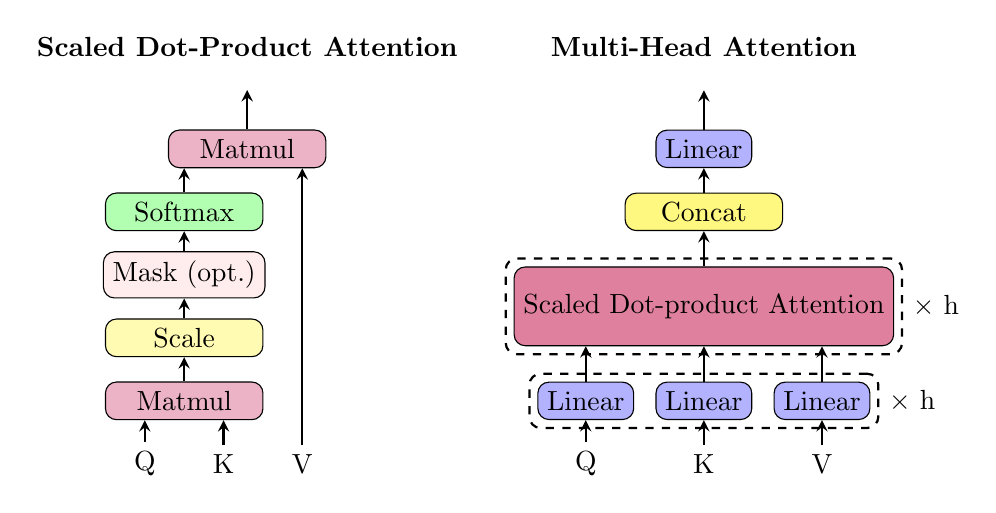
\begin{tikzpicture}[node distance=0.8cm]

\tikzstyle{matmul} = [rectangle,rounded corners, minimum width=2cm , text centered, draw=black, fill=purple!30]
\tikzstyle{softmax} = [rectangle,rounded corners, minimum width=2cm , text centered, draw=black, fill=green!30]
\tikzstyle{mask} = [rectangle,rounded corners, minimum width=2cm , text centered, draw=black, fill=pink!30]
\tikzstyle{sca} = [rectangle, rounded corners, minimum width=2cm ,text centered, draw=black, fill=yellow!30]
\tikzstyle{action} = [rectangle, rounded corners, minimum width=2cm ,text centered, draw=black, fill=red!30]
\tikzstyle{arrow} = [thick,->,>=stealth]

\tikzstyle{linear} = [rectangle, rounded corners, minimum width=1cm ,text centered, draw=black, fill=blue!30]
\tikzstyle{dot-prod} = [rectangle, rounded corners, minimum width=2cm,minimum height = 1cm ,text centered, draw=black, fill=purple!50]
\tikzstyle{concat} = [rectangle, rounded corners, minimum width=2cm ,text centered, draw=black, fill=yellow!50]



% Define nodes
\node (matmul1) [matmul]{Matmul};
\node (softmax)[softmax, below of = matmul1, xshift = -0.8cm]{Softmax};
\node (mask) [mask, below of=softmax]{Mask (opt.)};
\node (scale) [sca, below of=mask]{Scale};
\node (matmul2) [matmul, below of=scale]{Matmul};
\node (q) [below of=matmul2, xshift=-0.5cm]{Q};
\node (k) [below of=matmul2, xshift=0.5cm]{K};
\node (v) [below of=matmul2, xshift=1.5cm]{V};


% Draw arrows
\draw [arrow] (matmul1.north) -- ([yshift=0.5cm]matmul1.north);
\draw [arrow] (softmax.north) -- ([xshift=-0.8cm]matmul1.south);
\draw [arrow] (mask.north) -- (softmax.south);
\draw [arrow] (scale.north) -- (mask.south);
\draw [arrow] (matmul2.north) -- (scale.south);
\draw [arrow] (q.north) -- ([xshift=-0.5cm]matmul2.south);
\draw [arrow] (k.north) -- ([xshift=0.5cm]matmul2.south);
\draw [arrow] (v.north) -- ([xshift=0.7cm]matmul1.south);


% MHA 
\node (linear1) [linear, right of = matmul1, xshift = 5cm] {Linear};
\node (concat) [concat, below of = linear1] {Concat};
\node (dot-prod) [dot-prod, below of = concat,yshift= -0.4cm] {Scaled Dot-product Attention};
\node (linear2) [linear, below of = dot-prod, xshift = -1.5cm, yshift = -0.4cm] {Linear};
\node (linear3) [linear, below of = dot-prod, yshift = -0.4cm] {Linear};
\node (linear4) [linear, below of = dot-prod, xshift = 1.5cm, yshift = -0.4cm] {Linear};
\node (q2) [below of=linear2]{Q};
\node (k2) [below of=linear3]{K};
\node (v2) [below of=linear4]{V};

% MHA arrow
\draw [arrow] (q2) -- (linear2);
\draw [arrow] (k2) -- (linear3);
\draw [arrow] (v2) -- (linear4);
\draw [arrow] (linear2.north) -- ([xshift=-1.5cm]dot-prod.south);
\draw [arrow] (linear3.north) -- (dot-prod.south);
\draw [arrow] (linear4.north) -- ([xshift=1.5cm]dot-prod.south);
\draw [arrow] (dot-prod) -- (concat);
\draw [arrow] (concat) -- (linear1);
\draw [arrow] (linear1.north) -- ([yshift=0.5cm]linear1.north);

% MHA * h
\node[draw, thick, dashed, rounded corners, fit=(dot-prod), inner sep=0.1cm, label=right:{$\times$ h}] {};
\node[draw, thick, dashed, rounded corners, fit=(linear2)(linear3)(linear4), inner sep=0.1cm, label=right:{$\times$ h}] {};


% Title
\node (dot_t) [above of = matmul1,yshift=0.5cm] {\textbf{Scaled Dot-Product Attention}};
\node (mha) [above of = linear1,yshift=0.5cm] {\textbf{Multi-Head Attention}};



\end{tikzpicture}
        \caption{Illustration du mécanisme d'auto-attention : A droite le mécanisme complet, a gauche le \textit{Scaled Dot-product Attention}}
    \end{figure}
    
\end{frame}

\begin{frame}{Annexes \ref{ap:lora} : Low Rank Adaptation (LoRA)}
    \label{ap:lora}
    \begin{figure}
        \centering
        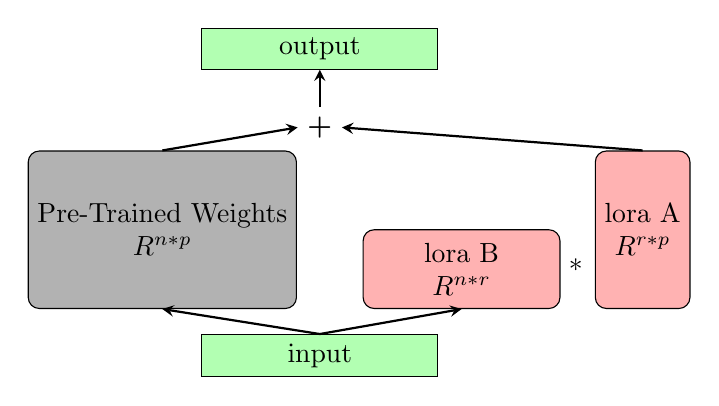
\begin{tikzpicture}[node distance=1.8cm]
    % Define block styles
    \tikzstyle{weights} = [rectangle,rounded corners, minimum width=2.5cm, minimum height=2cm, text centered, draw=black, fill=black!30]
    \tikzstyle{lora_a} = [rectangle,rounded corners, minimum width=1cm, minimum height=2cm, text centered, draw=black, fill=red!30]
    \tikzstyle{lora_b} = [rectangle,rounded corners, minimum width=2.5cm, minimum height=1cm, text centered, draw=black, fill=red!30]
    \tikzstyle{vector} = [rectangle, minimum width=3cm, minimum height=0.5cm, text centered, draw=black, fill=green!30]
    \tikzstyle{arrow} = [thick,->,>=stealth]
    
    % Define nodes
    \node (weights) [weights, align=center]{Pre-Trained Weights \\ $\mathbb{R}^{n*p}$};
    \node (lora_B) [lora_b, right of=weights,xshift=2cm,yshift=-0.5cm, align=center]{lora B\\ $\mathbb{R}^{n*r}$};
    \node (mul) [right of = lora_B,xshift=-0.35cm]{*};
    \node (lora_A) [lora_a, right of=lora_B,xshift=0.5cm,yshift=0.5cm, align=center]{lora A\\$\mathbb{R}^{r*p}$};
    \node (input) [vector,below of = weights, xshift = 2cm,yshift=+0.2cm]{input};
    \node (plus) [above of = weights, xshift = 2cm,yshift=-0.5cm]{\textbf{+}};
    \node (output) [vector,above of = plus,yshift=-0.8cm]{output};
    
    
    
    
    % Draw arrows
    \draw [arrow] (input.north) -- (weights.south);
    \draw [arrow] (input.north) -- (lora_B.south);
    \draw [arrow] (weights.north) -- (plus.west);
    \draw [arrow] (lora_A.north) -- (plus.east);
    \draw [arrow] (plus) -- (output);
    
    
    \end{tikzpicture}
        \caption{Illustration de l'application du Low Rank Adaptation (LoRA)}
    \end{figure}
    
\end{frame}

%%%%%%%%%%%%%%%%%%%%%%%%%%%%%%%%%%%%%%%%%%%%%%%%%%%%%%% 

\end{document}

%%%%%%%%%%%%%%%%%%%%%%%%%%%%%%%%%%%%%%%%%%%%%%%%%%%%%%%
%%
%%%%%%%%%%%%%%%%%%%%%%%%%%%%%%%%%%%%%%%%%%%%%%%%%%%%%%%

